\begin{frame}
      \titlepage

        \centering
          Grafi di assemblaggio
\end{frame}


\begin{frame}[fragile]
\frametitle{Assemblaggio di genomi}
\begin{block}{Tecnologie}
\begin{itemize}
\item
Porzioni di genoma chiamate \alert{read}
\item
50--10000bp (base pairs)
\item
spesso in coppie (\alert{mate pairs})
\item
posizione originaria ignota
\end{itemize}
\end{block}

\begin{block}{Obiettivo}
Ricostruire il genoma: circa 3 miliardi bp
\end{block}
\end{frame}

\begin{frame}[fragile]
\frametitle{Evoluzione tecnologica}
\includegraphics[width=0.7\textwidth]{figures/Developments_in_next_generation_sequencing.jpg}
\end{frame}

\begin{frame}[fragile]
\frametitle{Mate pairs}
\begin{minipage}{.48\textwidth}
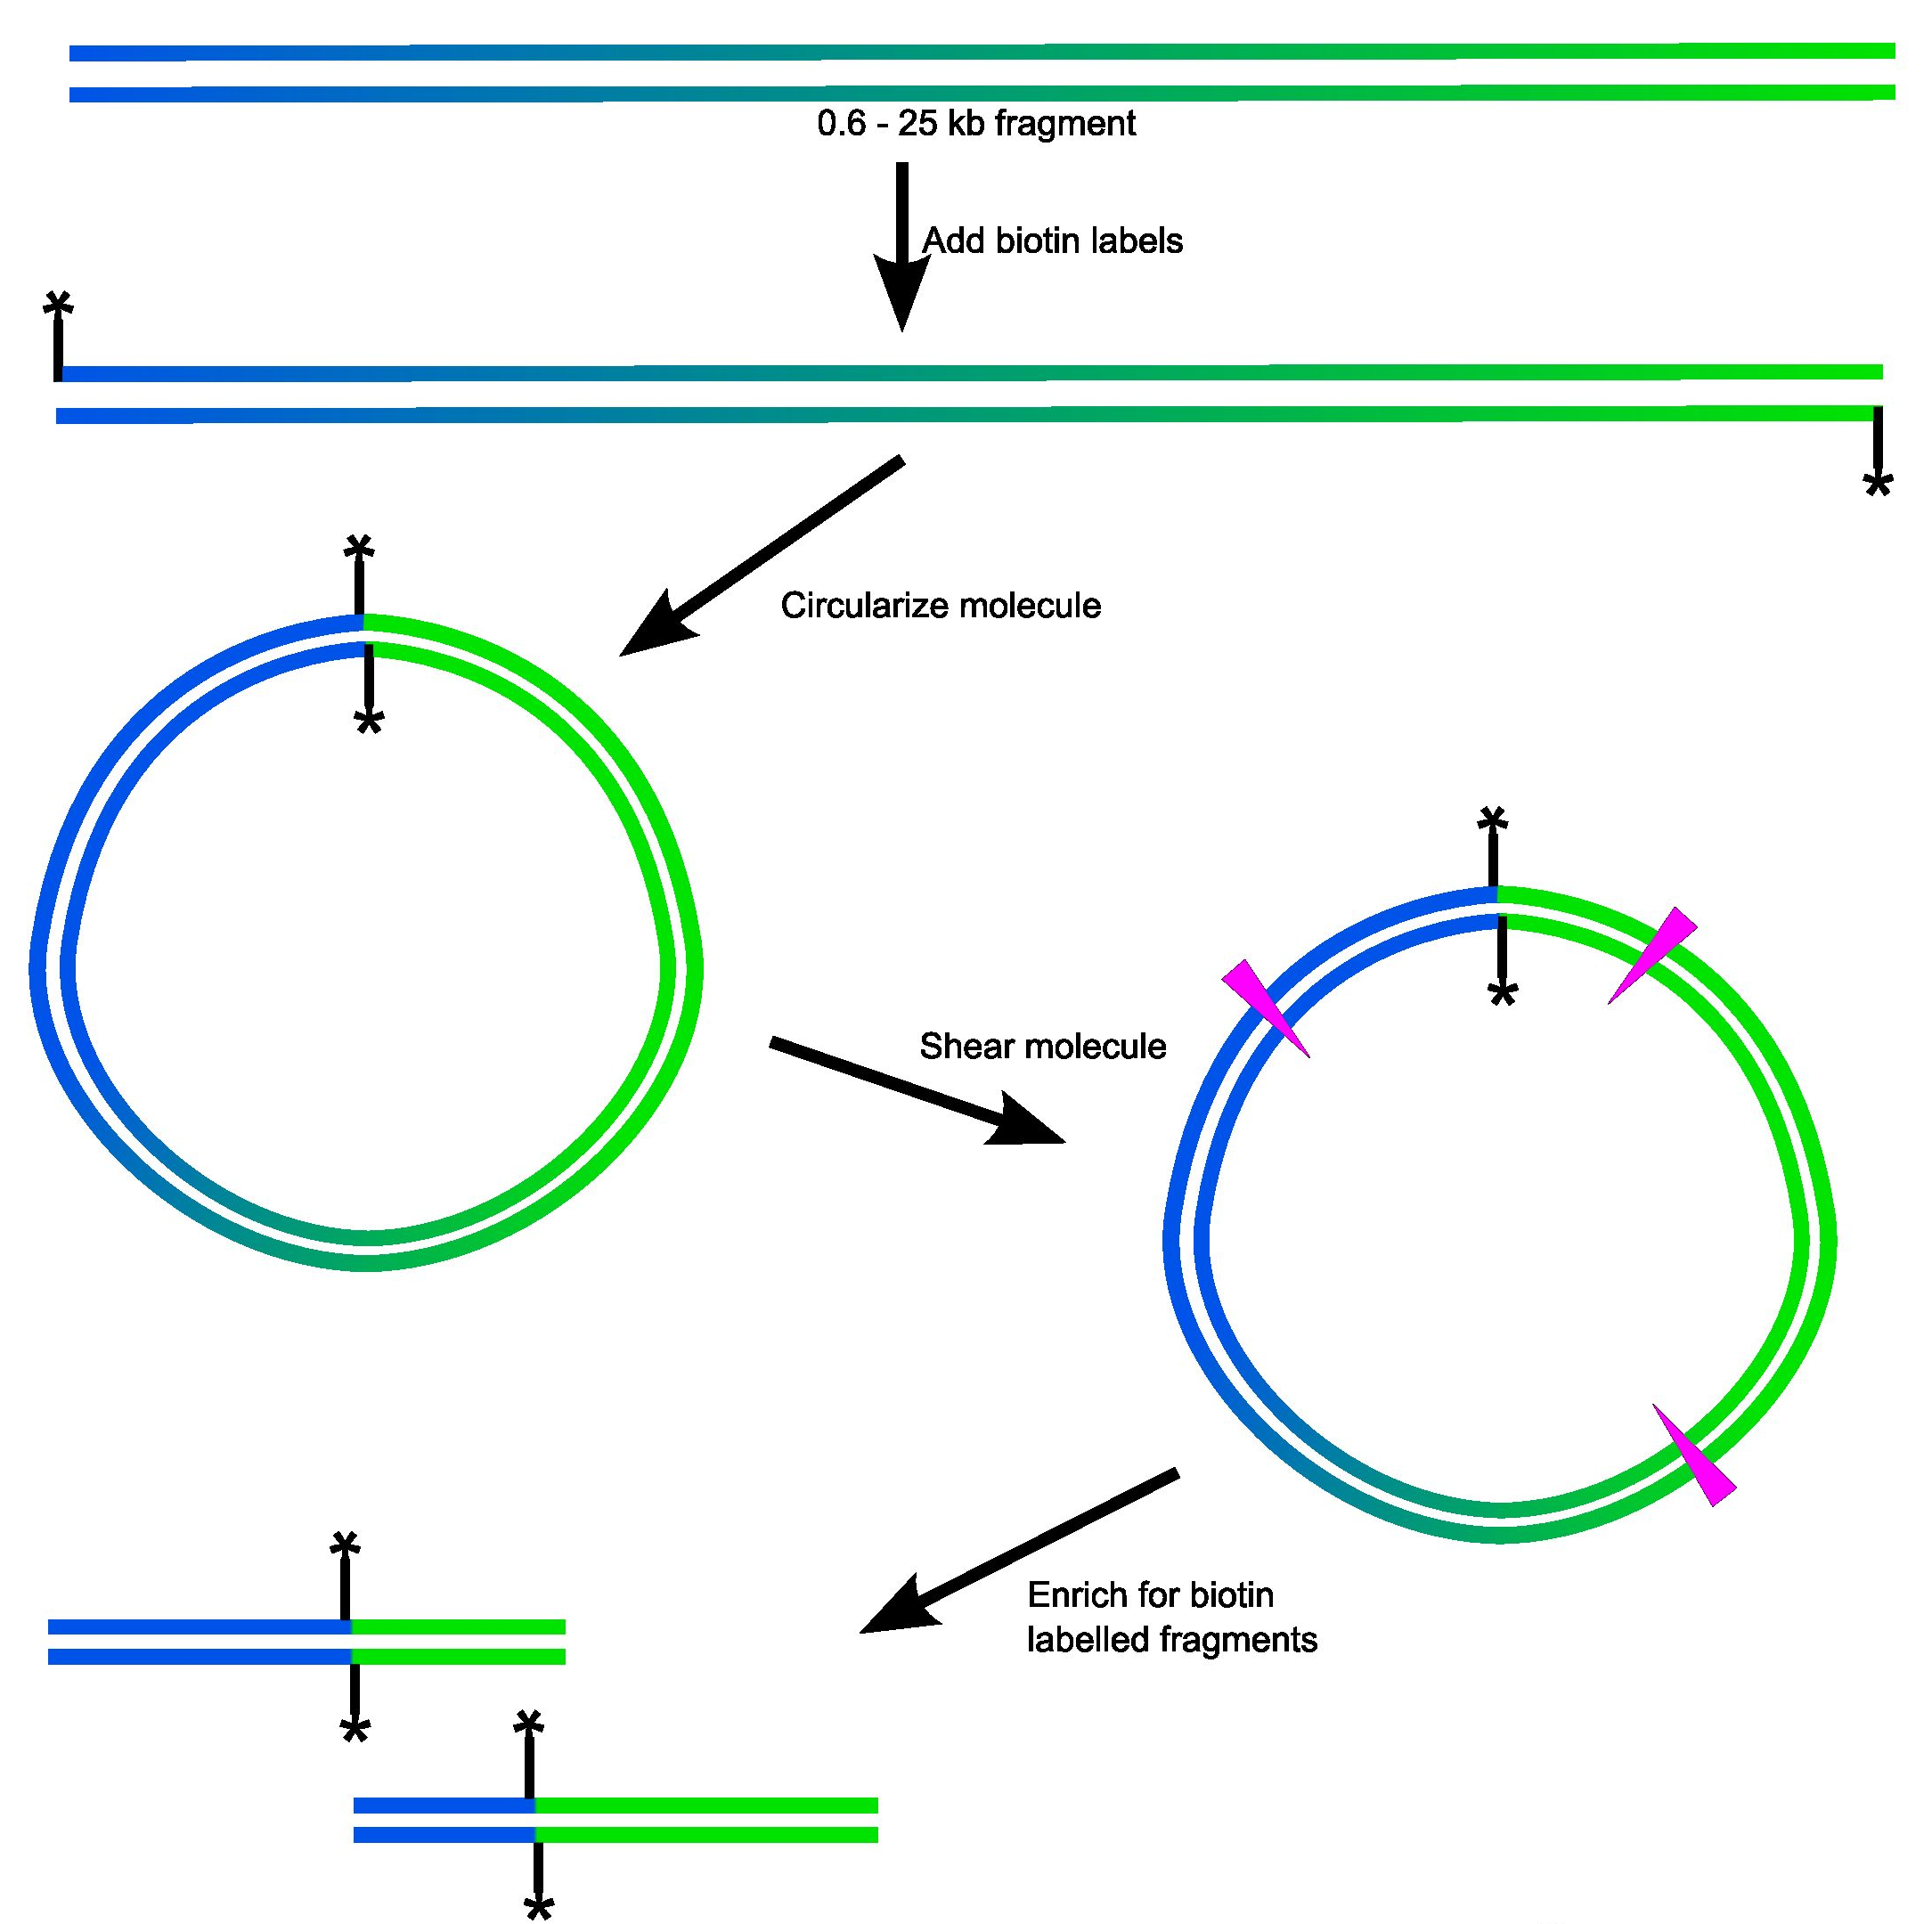
\includegraphics[width=\textwidth]{figures/mate-pairs-1.png}
\end{minipage}\hfill%
\begin{minipage}{.48\textwidth}
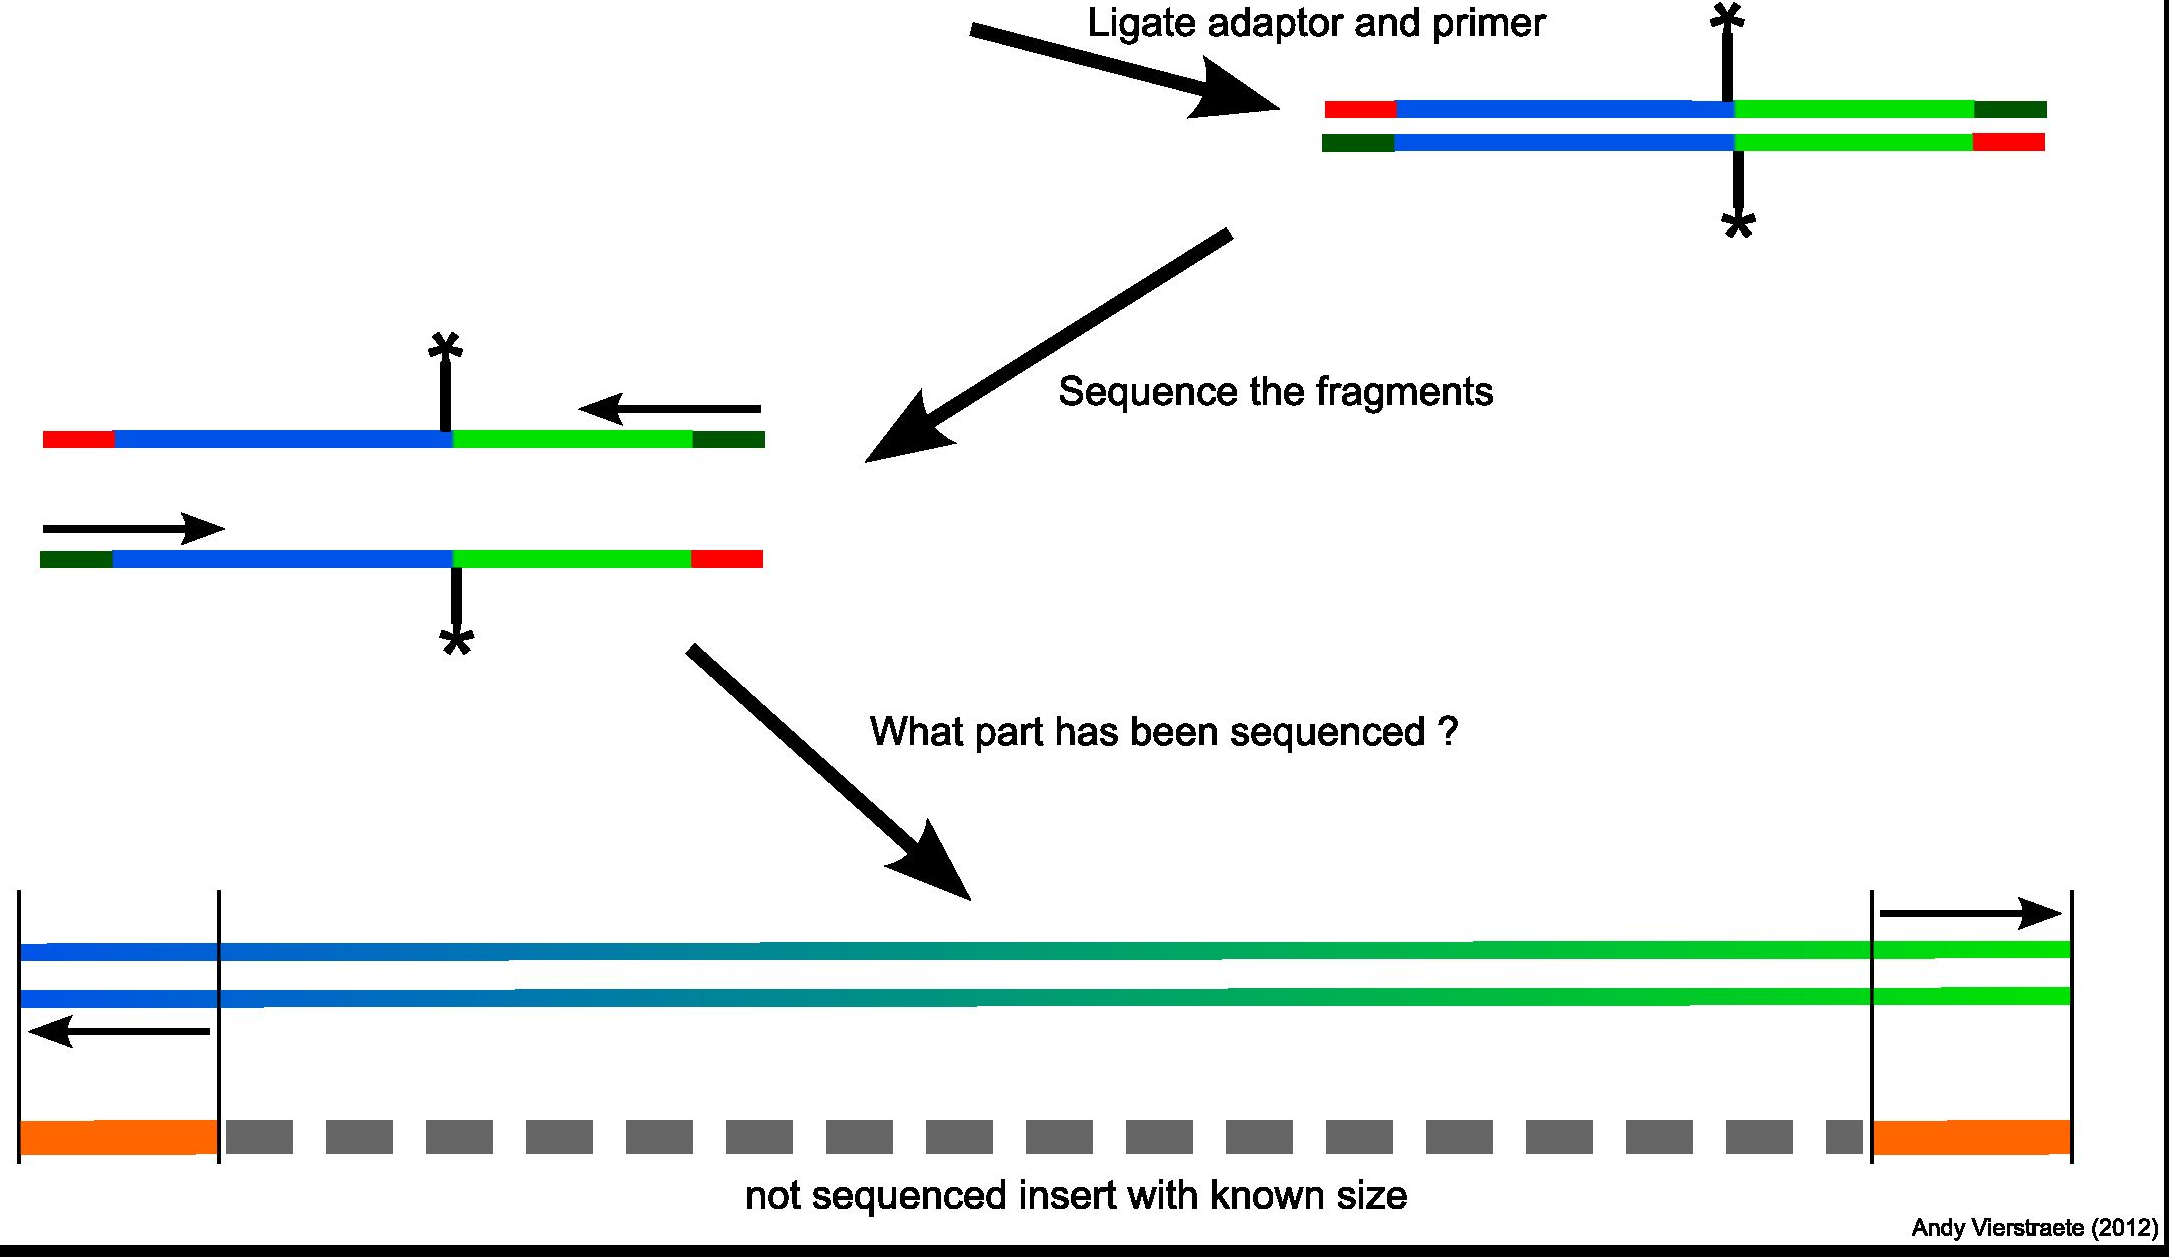
\includegraphics[width=\textwidth]{figures/mate-pairs-2.png}
\end{minipage}
\end{frame}

\begin{frame}[fragile]
\frametitle{Regola 1}

Suffisso di una read può essere prefisso di un'altra read: overlap

\begin{block}{Overlap --- sovrapposizione}
\begin{Verbatim}
    TCTATATCTCGGCTCTAGG 
        ||||||| ||||||| 
        TATCTCGACTCTAGGCC
\end{Verbatim}        
\end{block}

\begin{block}{Probabile motivo}
\begin{Verbatim}
    TCTATATCTCGGCTCTAGG 
GGCGTCTATATCTCGGCTCTAGGCCCTCATTTTTT 
        TATCTCG\alert{A}CTCTAGGCC
        \end{Verbatim}
\end{block}

Errore oppure organismi diploidi
\end{frame}

\begin{frame}[fragile]
\frametitle{Grafo di overlap}
				\begin{block}{Read}
\begin{tikzpicture}
\node[rectangle, fill=blue!95, font=\scriptsize]	(s1) at (0,0) {ACGTGTG};
\node[rectangle, fill=blue!90, font=\scriptsize]	(s2) [right= 10pt of s1] {CGTGTGC};
\node[rectangle, fill=blue!90, font=\scriptsize]	(s3) [right= 10pt of s2]{GTGCCA};
\node[rectangle, fill=blue!99, font=\scriptsize]	(s4) [right= 10pt of s3]{CCACG};
\end{tikzpicture}
\end{block}

Arco fra tutte le coppie di read con overlap abbastanza lungo

\begin{block}{Grafo}
					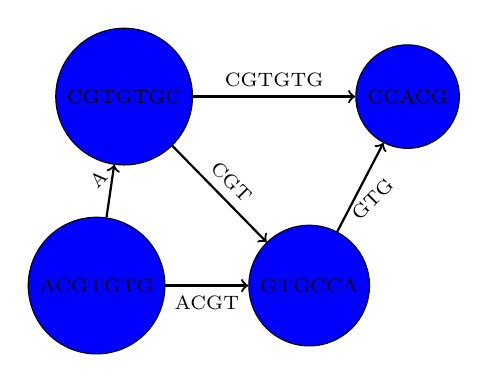
\begin{tikzpicture}
					\node[draw, fill=blue, circle, font=\scriptsize, minimum size=1cm] (k1) at (0,-2.8) {ACGTGTG};
					\node[draw, fill=blue, circle, font=\scriptsize, minimum size=1cm] (k2) at (0.35,-0.4) {CGTGTGC};
					\node[draw, fill=blue, circle, font=\scriptsize, minimum size=1cm] (k3) at (2.7,-2.8) {GTGCCA};
					\node[draw, fill=blue, circle, font=\scriptsize, minimum size=1cm] (k4) at (3.95,-0.4) {CCACG};
					
					\draw[->, thick] (k1) to node[rotate=45, font=\scriptsize, above] {A} (k2);
					\draw[->, thick] (k2) to node[rotate=-45, font=\scriptsize, above] {CGT} (k3);
					\draw[->, thick] (k3) to node[rotate=45, font=\scriptsize, below] {GTG} (k4);
					
					\draw[->, thick] (k1) to node[font=\scriptsize, below] {ACGT} (k3);
					\draw[->, thick] (k2) to node[font=\scriptsize, above] {CGTGTG}(k4);
					\end{tikzpicture}
          \end{block}
                  \end{frame}
        

\begin{frame}[fragile]
\frametitle{String Graph}
				\begin{block}{Read}
\begin{tikzpicture}
\node[rectangle, fill=blue!95, font=\scriptsize]	(s1) at (0,0) {ACGTGTG};
\node[rectangle, fill=blue!90, font=\scriptsize]	(s2) [right= 10pt of s1] {CGTGTGC};
\node[rectangle, fill=blue!90, font=\scriptsize]	(s3) [right= 10pt of s2]{GTGCCA};
\node[rectangle, fill=blue!99, font=\scriptsize]	(s4) [right= 10pt of s3]{CCACG};
\end{tikzpicture}
\end{block}

Si rimuovono gli archi transitivi dal grafo di overlap

\begin{block}{Grafo}
					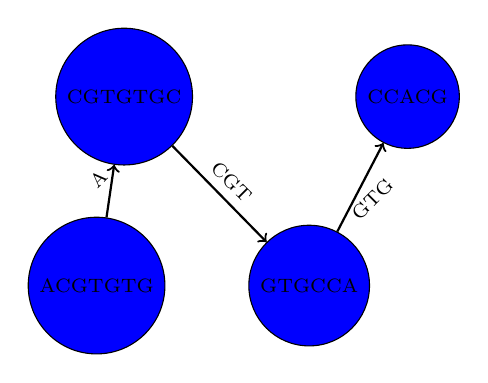
\begin{tikzpicture}
					\node[draw, fill=blue, circle, font=\scriptsize, minimum size=1cm] (k1) at (0,-2.8) {ACGTGTG};
					\node[draw, fill=blue, circle, font=\scriptsize, minimum size=1cm] (k2) at (0.35,-0.4) {CGTGTGC};
					\node[draw, fill=blue, circle, font=\scriptsize, minimum size=1cm] (k3) at (2.7,-2.8) {GTGCCA};
					\node[draw, fill=blue, circle, font=\scriptsize, minimum size=1cm] (k4) at (3.95,-0.4) {CCACG};
					
					\draw[->, thick] (k1) to node[rotate=45, font=\scriptsize, above] {A} (k2);
					\draw[->, thick] (k2) to node[rotate=-45, font=\scriptsize, above] {CGT} (k3);
					\draw[->, thick] (k3) to node[rotate=45, font=\scriptsize, below] {GTG} (k4);
					
					\end{tikzpicture}
				\end{block}
        \end{frame}

        
\begin{frame}[fragile]
\frametitle{Shortest superstring}
\begin{block}{Istanza}
Insieme $\mathcal{S} = \{s_{1}, \ldots , s_{n}\}$ di stringhe
\end{block}
\begin{block}{Soluzioni ammissibili}
Superstring $T$ di $\mathcal{S}$.
Ogni $s_{i}$ è sottostringa di $T$
\end{block}

\begin{block}{Funzione obiettivo}
$|T|$
\end{block}

$T$ è il genoma assemblato, $\mathcal{S}$ le read

\begin{block}{Problema}
Regioni ripetute
\end{block}
\end{frame}


\begin{frame}[fragile]
\frametitle{Algoritmo ingordo}
\begin{block}{Algoritmo}
\begin{enumerate}
\item
Fondere le due stringhe con massimo overlap
\item
Finchè non rimane una stringa sola
\end{enumerate}
\end{block}
\end{frame}

\begin{frame}[fragile]
\frametitle{Esempio: a\_long\_long\_long\_time}
\begin{enumerate}
\item 
ng\_lon \_long\_ a\_long long\_l ong\_ti ong\_lo long\_t g\_long 
\alert{g\_time ng\_tim}
\item
  ng\_time ng\_lon 
\alert{\_long\_}
 a\_long long\_l ong\_ti ong\_lo long\_t 
\alert{g\_long}
\item
  ng\_time g\_long\_ ng\_lon a\_long long\_l 
\alert{ong\_ti}
 ong\_lo 
\alert{long\_t}
\item
  ng\_time long\_ti g\_long\_ 
\alert{ng\_lon}
 a\_long long\_l 
\alert{ong\_lo}
\item
\alert{ng\_time}
 ong\_lon 
\alert{long\_ti}
 g\_long\_ a\_long long\_l 
\item
\alert{ong\_lon}
 long\_time g\_long\_ a\_long 
long\_l\alert{}
\item
  long\_lon 
\alert{long\_time g\_long\_}
 a\_long 
\item
\alert{long\_lon g\_long\_time}
 a\_long 
\item
\alert{long\_long\_time a\_long}
\item
  a\_long\_long\_time
  \end{enumerate}
  \end{frame}

  
\begin{frame}[fragile]
\frametitle{Problema del commesso viaggiatore (TSP)}
\begin{block}{Istanza}
Grafo orientato $G=\langle  V,A \rangle$, con archi pesati $w:A \mapsto \mathbb{Q}^{+}$
\end{block}
\begin{block}{Soluzioni ammissibili}
Permutazione $\Pi=\langle  \pi_{1}, \ldots,  \pi_{n} \rangle$ of $V$
\end{block}
\begin{block}{Funzione obiettivo}
$w(\pi_{n},\pi_{1}) + \sum_{i=1}^{n} w(\pi_{i},\pi_{i+1})$
\end{block}
\begin{itemize}
\item
Una soluzione è un percorso che tocca ogni città esattamente una volta e torna
al punto di partenza
\item
Il costo è il peso totale di tutti gli archi attraversati
\item
NP-completo\uncover<2>{\alert{, ma risolvibile in pratica}}
\end{itemize}
\end{frame}

\begin{frame}[fragile]
\frametitle{Superstringa più corta e TSP}
\begin{block}{Similarità}
1 read = 1 città
\end{block}
\begin{block}{Differenze}
\begin{itemize}
\item
assemblaggio $\neq$ ciclo
\item
lunghezza stringa $\neq$ costo percorso TSP
\end{itemize}
\end{block}

\uncover<2>{
\begin{block}{Proprietà}
$|\mathcal{S}| = \sum_{i=1}^{n}|s_{i}| - \sum_{i=1}^{n-1}|ov(s_{i}, s_{i+1})|$, dove
$ov(\cdot,\cdot)$ è la lunghezza della sovrapposizione fra le stringhe
\end{block}}
\end{frame}

\begin{frame}[fragile]
\frametitle{Grafo di overlap --- TSP}
				\begin{block}{Read}
\begin{tikzpicture}
\node[rectangle, fill=blue!95, font=\scriptsize]	(s1) at (0,0) {ACGTGTG};
\node[rectangle, fill=blue!90, font=\scriptsize]	(s2) [right= 10pt of s1] {CGTGTGC};
\node[rectangle, fill=blue!90, font=\scriptsize]	(s3) [right= 10pt of s2]{GTGCCA};
\node[rectangle, fill=blue!99, font=\scriptsize]	(s4) [right= 10pt of s3]{CCACG};
\end{tikzpicture}
\end{block}


\begin{block}{Grafo}
					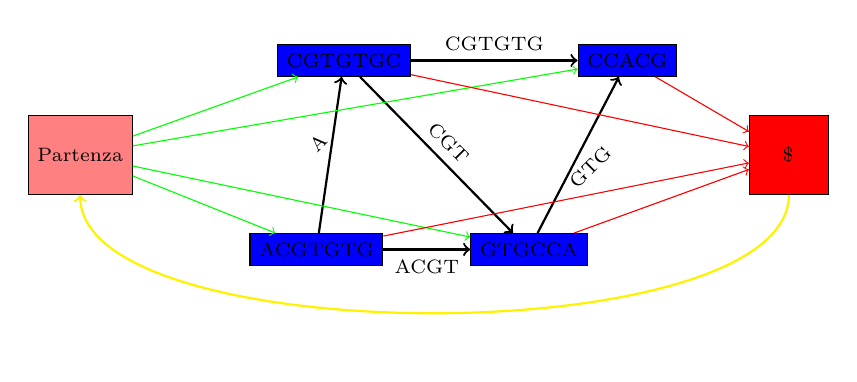
\begin{tikzpicture}
					\node[draw, fill=red!50, rectangle, font=\scriptsize, minimum size=1cm] (p0) at (-2,-1.6) {Partenza};
					\node[draw, fill=red, rectangle, font=\scriptsize, minimum size=1cm] (p1) at (7,-1.6) {\$};

					\node[draw, fill=blue, rectangle, font=\scriptsize] (k1) at (1,-2.8) {ACGTGTG};
					\node[draw, fill=blue, rectangle, font=\scriptsize] (k2) at (1.35,-0.4) {CGTGTGC};
					\node[draw, fill=blue, rectangle, font=\scriptsize] (k3) at (3.7,-2.8) {GTGCCA};
					\node[draw, fill=blue, rectangle, font=\scriptsize] (k4) at (4.95,-0.4) {CCACG};
					
					\draw[->, thick] (k1) to node[rotate=45, font=\scriptsize, above] {A} (k2);
					\draw[->, thick] (k2) to node[rotate=-45, font=\scriptsize, above] {CGT} (k3);
					\draw[->, thick] (k3) to node[rotate=45, font=\scriptsize, below] {GTG} (k4);
					
					\draw[->, thick] (k1) to node[font=\scriptsize, below] {ACGT} (k3);
					\draw[->, thick] (k2) to node[font=\scriptsize, above] {CGTGTG}(k4);

					\draw[->, green] (p0) to (k1);
					\draw[->, green] (p0) to (k2);
					\draw[->,	green] (p0) to (k3);
					\draw[->, green] (p0) to (k4);

					\draw[->, red] (k1) to (p1);
					\draw[->, red]	(k2) to (p1);
					\draw[->, red]	(k3) to (p1);
					\draw[->, red]	(k4) to (p1);

          \draw[->, yellow, thick]	(p1.south)  .. controls +(down:20mm) and +(down:20mm)
.. (p0.south);
\end{tikzpicture}
          \end{block}
                  \end{frame}


\begin{frame}[fragile]
\frametitle{Overlay --- Layout --- Consensus}
\begin{block}{Passi}
\begin{enumerate}
\item
Overlap: calcolare le sovrapposizioni e costruire il grafo.
Usare suffix array (esatto) o programmazione dinamica (errori).
\item
Layout: Fondere i cammini per ottenere i  \alert{contigs}.
Le ripetizioni (branching nodes) vengono rimosse.
\item
Consensus: calcola i nucleotidi
\end{enumerate}
\end{block}
\end{frame}

\begin{frame}[fragile]
\frametitle{Reverse and complement}
\begin{itemize}
\item
Non si conosce lo strand
\item
Versione canonica (minima fra $x$ e revcomp$(x)$
\item
complica il calcolo degli overlap
\end{itemize}
\end{frame}

\begin{frame}[fragile]
\frametitle{SBH}
\begin{block}{DNA array}
\begin{itemize}
\item
Tecnologia vecchia
\item
Per ogni $k$-mero, si conosce se appare nel genoma
\item
$k\approx 8$
\end{itemize}
\end{block}

\begin{block}{Procedura}
\begin{enumerate}
\item
Ogni $k$-mero viene diviso in $(k-1)$-meri
\item
Un vertice per ogni $(k-1)$-mero
\item
Un arco per ogni $k$-mero
\end{enumerate}
\end{block}
\begin{block}{Adesso}
Stessa procedura, a partire dai read
\end{block}

\end{frame}



\begin{frame}[t, fragile]
	\frametitle{Grafo di de Bruijn}
		\begin{columns}
	\begin{column}[t]{0.48\textwidth}
              	\begin{center}
				\begin{block}{Read}
\begin{tikzpicture}
\node[rectangle, fill=blue!95, font=\scriptsize]	(s1) at (0,0) {ACGTGTG};
\node[rectangle, fill=blue!90, font=\scriptsize]	(s2) [right= 10pt of s1] {CGTGTGC};
\node[rectangle, fill=blue!90, font=\scriptsize]	(s3) [right= 10pt of s2]{GTGCCA};
\node[rectangle, fill=blue!99, font=\scriptsize]	(s4) [right= 10pt of s3]{CCACG};
\end{tikzpicture}
\end{block}

															\begin{block}{de Bruijn graphs}
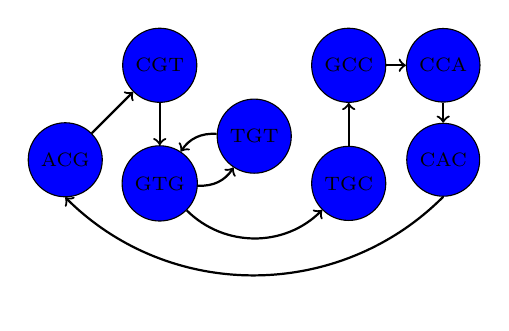
\begin{tikzpicture}
\node[draw, fill=blue, circle, font=\scriptsize] (k0) at (0,-2.6) {ACG};
\node[draw, fill=blue, circle, font=\scriptsize] (k1) at (1.2,-1.4) {CGT};
\node[draw, fill=blue, circle, font=\scriptsize] (k2) at (1.2,-2.9) {GTG};
\node[draw, fill=blue, circle, font=\scriptsize] (k3) at (2.4,-2.3) {TGT};
\node[draw, fill=blue, circle, font=\scriptsize] (k4) at (3.6,-2.9) {TGC};

\node[draw, fill=blue, circle, font=\scriptsize] (k5) at (3.6,-1.4) {GCC};
\node[draw, fill=blue, circle, font=\scriptsize] (k6) at (4.8,-1.4) {CCA};
\node[draw, fill=blue, circle, font=\scriptsize] (k7) at (4.8,-2.6) {CAC};
%						 \node[draw, circle, font=\scriptsize] (k7) at (4,-2.0) {};

\draw[->, thick] (k0) to (k1);
\draw[->, thick] (k1) to (k2);
\draw[->, thick] (k3) to[bend right] (k2);
\draw[->, thick] (k2) to[bend right] (k3);
\draw[->, thick] (k2) to[bend right=45] (k4);
\draw[->, thick] (k4) to (k5);
% \draw[->, thick] (k2) to[bend right=45] (k4);
% \draw[->, thick] (k4) to (k5);
\draw[->, thick] (k5) to (k6);
\draw[->, thick] (k6) to (k7);
\draw[->, thick] (k7.south) to[bend left=45] (k0.south);
\end{tikzpicture}
\end{block}


\end{center}
\end{column}
\begin{column}[t]{0.48\textwidth}
				\begin{block}{$4$-meri --- $3$-meri --- distinti}
\begin{tikzpicture}
\node[rectangle, fill=blue!85, font=\scriptsize]	(s1a) at (0,0)           {ACGT};
\node[rectangle, fill=blue!85, font=\scriptsize]	(s4b) [below= 1pt of s1a]{CACG};
\node[rectangle, fill=blue!85, font=\scriptsize]	(s4a) [below= 1pt of s4b]{CCAC};
\node[rectangle, fill=blue!85, font=\scriptsize]	(s1b) [below= 1pt of s4a]{CGTG};
\node[rectangle, fill=blue!85, font=\scriptsize]	(s3c) [below= 1pt of s1b]{GCCA};
\node[rectangle, fill=blue!85, font=\scriptsize]	(s3a) [below= 1pt of s3c]{GTGC};
\node[rectangle, fill=blue!85, font=\scriptsize]	(s1c) [below= 1pt of s3a]{GTGT};
\node[rectangle, fill=blue!85, font=\scriptsize]	(s3b) [below= 1pt of s1c]{TGCC};
\node[rectangle, fill=blue!85, font=\scriptsize]	(s1d) [below= 1pt of s3b]{TGTG};


\node[rectangle, fill=blue!45, font=\scriptsize]	(l1a) at (1.9,0)           {ACG};
\node[rectangle, fill=blue!45, font=\scriptsize]	(l4b) [below= 1pt of l1a]{CAC};
\node[rectangle, fill=blue!45, font=\scriptsize]	(l4a) [below= 1pt of l4b]{CCA};
\node[rectangle, fill=blue!45, font=\scriptsize]	(l1b) [below= 1pt of l4a]{CGT};
\node[rectangle, fill=blue!45, font=\scriptsize]	(l3c) [below= 1pt of l1b]{GCC};
\node[rectangle, fill=blue!45, font=\scriptsize]	(l3a) [below= 1pt of l3c]{GTG};
\node[rectangle, fill=blue!45, font=\scriptsize]	(l1c) [below= 1pt of l3a]{GTG};
\node[rectangle, fill=blue!45, font=\scriptsize]	(l3b) [below= 1pt of l1c]{TGC};
\node[rectangle, fill=blue!45, font=\scriptsize]	(l1d) [below= 1pt of l3b]{TGT};

\node[rectangle, fill=blue!45, font=\scriptsize]	(r1a) [right= 1pt of l1a] {CGT};
\node[rectangle, fill=blue!45, font=\scriptsize]	(r4b) [below= 1pt of r1a]{ACG};
\node[rectangle, fill=blue!45, font=\scriptsize]	(r4a) [below= 1pt of r4b]{CAC};
\node[rectangle, fill=blue!45, font=\scriptsize]	(r1b) [below= 1pt of r4a]{GTG};
\node[rectangle, fill=blue!45, font=\scriptsize]	(r3c) [below= 1pt of r1b]{CCA};
\node[rectangle, fill=blue!45, font=\scriptsize]	(r3a) [below= 1pt of r3c]{TGC};
\node[rectangle, fill=blue!45, font=\scriptsize]	(r1c) [below= 1pt of r3a]{TGT};
\node[rectangle, fill=blue!45, font=\scriptsize]	(r3b) [below= 1pt of r1c]{GCC};
\node[rectangle, fill=blue!45, font=\scriptsize]	(r1d) [below= 1pt of r3b]{GTG};

\node[rectangle, fill=blue!45, font=\scriptsize]	(dl1a) at (5,0)           {ACG};
\node[rectangle, fill=blue!45, font=\scriptsize]	(dl4b) [below= 1pt of dl1a]{CAC};
\node[rectangle, fill=blue!45, font=\scriptsize]	(dl4a) [below= 1pt of dl4b]{CCA};
\node[rectangle, fill=blue!45, font=\scriptsize]	(dl1b) [below= 1pt of dl4a]{CGT};
\node[rectangle, fill=blue!45, font=\scriptsize]	(dl3c) [below= 1pt of dl1b]{GCC};
\node[rectangle, fill=blue!45, font=\scriptsize]	(dl3a) [below= 1pt of dl3c]{GTG};
\node[rectangle, fill=blue!25, color=blue!25, font=\scriptsize]	(dl1c) [below= 1pt of dl3a]{GTG};
\node[rectangle, fill=blue!45, font=\scriptsize]	(dl3b) [below= 1pt of dl1c]{TGC};
\node[rectangle, fill=blue!45, font=\scriptsize]	(dl1d) [below= 1pt of dl3b]{TGT};

\node[rectangle, fill=blue!25, color=blue!25, font=\scriptsize]	(dr1a) [right= 1pt of dl1a]{CGT};
\node[rectangle, fill=blue!25, color=blue!25, font=\scriptsize]	(dr4b) [below= 1pt of dr1a]{ACG};
\node[rectangle, fill=blue!25, color=blue!25, font=\scriptsize]	(dr4a) [below= 1pt of dr4b]{CAC};
\node[rectangle, fill=blue!25, color=blue!25, font=\scriptsize]	(dr1b) [below= 1pt of dr4a]{GTG};
\node[rectangle, fill=blue!25, color=blue!25, font=\scriptsize]	(dr3c) [below= 1pt of dr1b]{CCA};
\node[rectangle, fill=blue!25, color=blue!25, font=\scriptsize]	(dr3a) [below= 1pt of dr3c]{TGC};
\node[rectangle, fill=blue!25, color=blue!25, font=\scriptsize]	(dr1c) [below= 1pt of dr3a]{TGT};
\node[rectangle, fill=blue!25, color=blue!25, font=\scriptsize]	(dr3b) [below= 1pt of dr1c]{GCC};
\node[rectangle, fill=blue!25, color=blue!25, font=\scriptsize]	(dr1d) [below= 1pt of dr3b]{GTG};

\end{tikzpicture}
\end{block}
\end{column}
\end{columns}
\end{frame}

\begin{frame}[fragile]
\frametitle{Problemi su grafi}
\begin{block}{Ciclo Euleriano}
\begin{enumerate}
\item
Un assemblaggio valido è un cammino che attraversa \alert{ogni arco} esattamente una volta
\item
Cammino Euleriano
\end{enumerate}
\end{block}
\begin{block}{Ciclo Hamiltoniano}
\begin{enumerate}
\item
\'E un cammino che attraversa \alert{ogni vertice} esattamente una volta
\item
Caso particolare di TSP
\end{enumerate}
\end{block}
\begin{block}{Confronto}
Qual è più difficile da risolvere?
\end{block}
\end{frame}


\begin{frame}[fragile]
\frametitle{Grafi Euleriani}
\begin{block}{Definizione}
Sia $G=\langle  V,A \rangle$ un grafo orientato.
$G$ è semi-euleriano se esistono due vertici $s$, $t$ tali che $N^{-}_{G}(s) =
N^{+}_{G}(s) +1$,  $N^{-}_{G}(t) = N^{+}_{G}(v) -1$, mentre per ogni altro
vertice $w$,  $N^{-}_{G}(w) =N^{+}_{G}(w)$.
\end{block}

\begin{block}{Definizione}
Sia $G=\langle  V,A \rangle$ un grafo orientato.
$G$ è euleriano se $N^{-}_{G}(w) =N^{+}_{G}(w)$. per ogni
vertice.
\end{block}

\begin{block}{Teorema}
Un grafo connesso $G=\langle  V,A \rangle$ ha un cammino euleriano se e solo se $G$ è semi-euleriano.
$G$ ha un ciclo euleriano se e solo se $G$ è euleriano.
\end{block}
\end{frame}


\begin{frame}[fragile]
\frametitle{Grafi Euleriani 2}

\begin{block}{Teorema}
Sia $G=\langle  V,A \rangle$ un grafo semi-euleriano e sia $P$ un  cammino da $s$ a $t$.
Sia $G_{1}$ il grafo ottenuto da $G$ togliendo tutti gli archi di $P$.
Allora $G_{1}$ è euleriano.
\end{block}

\begin{block}{Teorema}
Sia $G=\langle  V,A \rangle$ un grafo euleriano e sia $C$ un ciclo di $G$.
Sia $G_{1}$ il grafo ottenuto da $G$ togliendo tutti gli archi di $C$.
Allora $G_{1}$ è euleriano.
\end{block}
\end{frame}

\begin{frame}[fragile]
\frametitle{Altre fasi}
\begin{itemize}
\item
bubble popping
\item
tip removal
\end{itemize}
\end{frame}

\begin{frame}[fragile]
\frametitle{Scaffolding}

\begin{itemize}
\item
Fondere contigs in scaffolds
\item
usando mate pairs
\item
anche con revcomp
\end{itemize}
\end{frame}


%%% Local Variables:
%%% TeX-PDF-mode: t
%%% TeX-master: "graphs-video"
%%% buffer-file-coding-system: utf-8
%%% End:
